\section{ADMIN}
    \subsection{Dashboard}
        Η κεντρική σελίδα του διαχειριστή περιλαμβάνει τέσσερα διαφορετικά modules: ένα με μια καταγραφή των items, των vehicles και των χρηστών,
            ένα όπου μπορούμε να δημιουργήσουμε ανακοινώσεις, ένα που μπορούμε να δημιουργήσουμε ένα λογαριασμό διασώστη, και ένα με την καταγραφή όλων των ανακοινώσεων.

        \vspace{-1em}
        \begin{figure}[H] \noindent \centering
            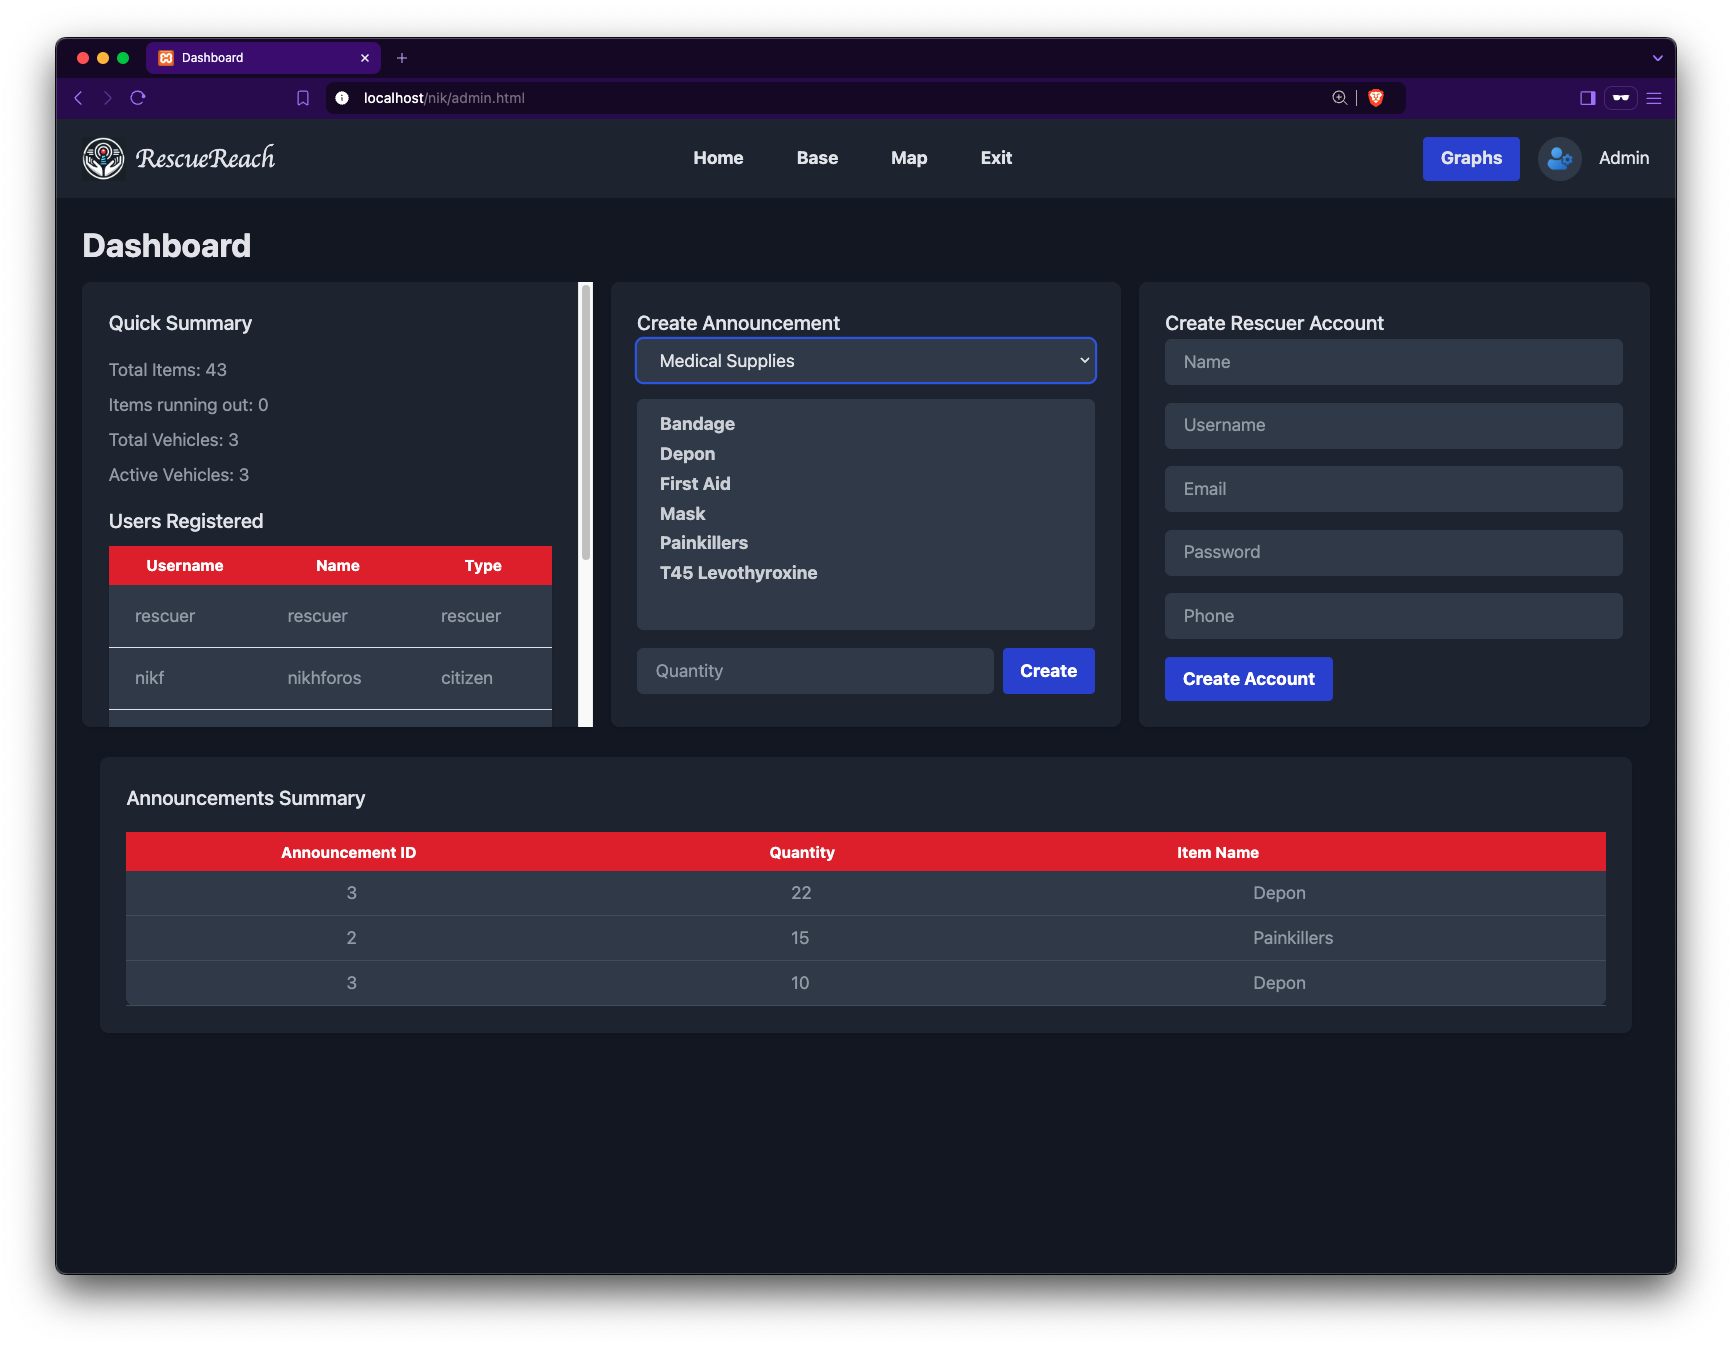
\includegraphics[width=0.9\textwidth]{img/admin-dashboard}
            \vspace{-1em}
            \caption{Dashboard admin}
        \end{figure}

        Το αρχείο \c{dashboard.js} χειρίζεται τη συγκεκριμένη σελίδα.
        Στην αρχή καλούνται όλες οι απαραίτητες συναρτήσεις για την εμφάνιση των διαφόρων modules.

        \subsubsection{Quick Summary}
            Η συνάρτηση \c{loadDashboardSummary()} στέλνει ένα AJAX request στο \c{summary.php}, ζητώντας τον συνολικό αριθμό των items (\c{#totalItems}),
                και τον αριθμό των items που τελειώνουν (\c{#lowStockItems}), και επιστρέφονται σε JSON μορφή.
            Αντίστοιχα η \c{fetchActiveVehicles()} στέλνει ένα AJAX request στο \c{active\_vehicles.php}, ζητώντας τον αριθμό των vehicles που είναι ενεργά (\c{#activeVehicles}).
            Η \c{registeredUsers()} δέχεται δεδομένα από το \c{registered\_users.php}, και μέσω της \c{populateTable()} εμφανίζει έναν πίνακα με τους εγγεγραμμένους χρήστες.

        \subsubsection{Create Announcement}
            Για τη φόρτωση των διαφορετικών κατηγοριών των items για τη δημιουργία της ανακοίνωσης, καλείται αρχικά η \c{loadCategoriesAndItems()}
            η οποία στέλνει ένα AJAX request στο \c{announchment.php}.
            Η PHP επιστρέφει ένα JSON αρχείο της μορφής:

            \begin{graycomment}
                \verb|{"categories": [id, name], "items": [id, name, category_id]}|
            \end{graycomment}

            Τα δεδομένα που επιστρέφονται χρησιμοποιούνται από τη \c{loadDashboardSummary()} για να γίνουν populate οι κατηγορίες της φόρμας.
            Αν ο χρήστης επιλέξει μια κατηγορία, η \c{filterItemsByCategory()} κάνει populate τη λίστα με τα αντίστοιχα items μέσω του JSON αρχείου.

            Όταν πατηθεί το κουμπί \textbf{Create}, αποθηκεύονται σε μεταβλητές τα επιλεγμένα items, όπως επίσης και το πλήθος τους
            και στέλνονται στη \c{insert\_announchment.php}, η οποία τα κάνει insert στη βάση.
            Σε περίπτωση επιτυχίας στέλνεται το αντίστοιχο μήνυμα.

        \subsubsection{Create Rescuer Account}
            Όταν πατηθεί το κουμπί \textbf{Create Account}, καλείται η \c{createRescuerAccount()} η οποία μέσω Promise δημιουργεί μεταβλητές για κάθε value της φόρμας,
                τις οποίες στέλνει μέσω AJAX request στο \c{create\_rescuer.php}.
            Η PHP ελέγχει αν υπάρχει ήδη τέτοιο username ή email, στέλνει κατάλληλα echos αν υπάρχουν, και αν δεν υπάρχουν κάνει insert τον νέο χρήστη στη βάση δεδομένων.

        \subsubsection{Announcements Summary}
            Ακολουθείται παρόμοια διαδικασία με τη δημιουργία του πίνακα των εγγεγραμμένων χρηστών.
            Χρησιμοποιείται η \c{loadAnnouchmentSummary()} σε συνδυασμό με τη \c{get\_ann.php}.

        \subsubsection{Graphs}
            Το κουμπί \textbf{Graphs} ενεργοποιεί ένα modal\footnote{με κατάλληλη προσθαφαίρεση κλάσεων του Tailwind} με στατιστικά γραφήματα για τα requests και τα offers.

            \begin{figure}[H] \noindent \centering
                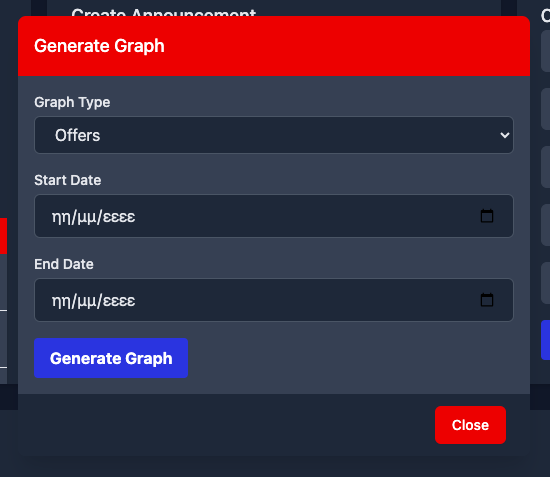
\includegraphics[width=0.4\textwidth]{img/admin-generate_graph}
                \caption{Generate Graph model}
            \end{figure}

            Δημιουργούνται οι σταθερές \c{startDate}, \c{endDate}, και \c{graphType}.
            Μέσω της \c{fetchGraphData()} δημιουργείται ένα Promise ανάλογα με το αν το \c{graphType} είναι offer ή request προς τα \verb|graph_<offers ή requests>.php?startDate=${startDate}&endDate=${endDate}|.

            Με το JSON αρχείο που επιστρέφεται σε κάθε περίπτωση, η \c{fetchGraphData()} μέσω της ChartJS δημιουργεί το αντίστοιχο γράφημα.

    \subsection{Base}
        \begin{figure}[H] \noindent \centering
            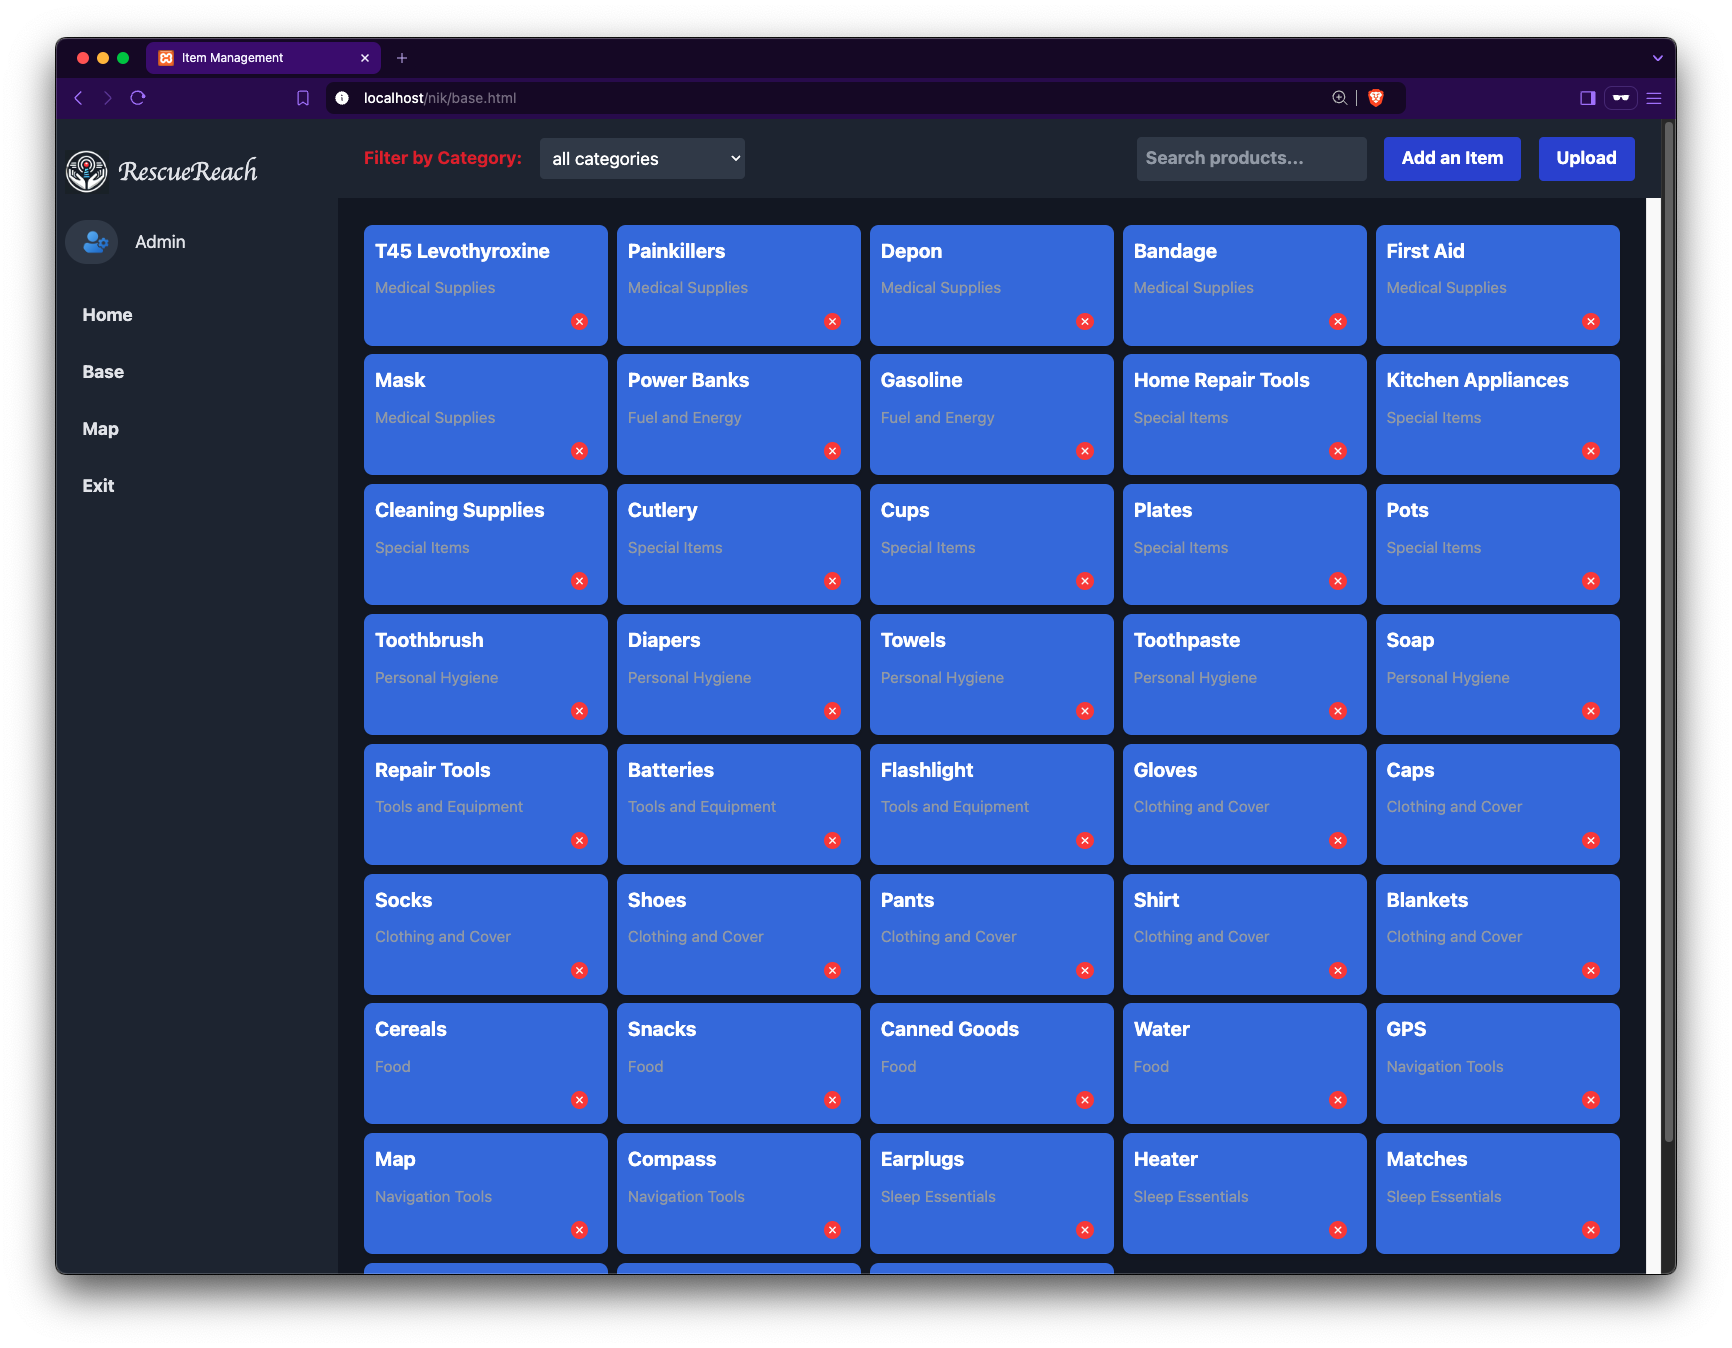
\includegraphics[width=0.8\textwidth]{img/admin-base}
            \caption{Σελίδα με τα αντικείμενα της Βάσης}
        \end{figure}

        Το αρχείο \c{base.js} χειρίζεται τη σελίδα \c{base.html}.
        Κατά την εμφάνιση της σελίδας δημιουργείται ένα AJAX request στο \c{item\_categories.php}, το οποίο επιστρέφει όλες τις κατηγορίες και τα προϊόντα της βάσης.
        Συγκεκριμένα επιστρέφεται ένα JSON αρχείο της μορφής:

        \begin{graycomment}
            \verb|{"categories": [...], "products": [id, name, category_id, category]}|
        \end{graycomment}

        Το population της σελίδας με τα αντικείμενα πραγματοποιείται μέσω της \c{updateProductGrid(products)}, η οποία περιέχει μια επανάληψη όπου προσθέτει divs στη HTML σελίδα.
        Περιέχονται Event Listeners για το hover και το click των διαφορετικών αντικειμένων.

        \begin{figure}[H] \noindent \centering
            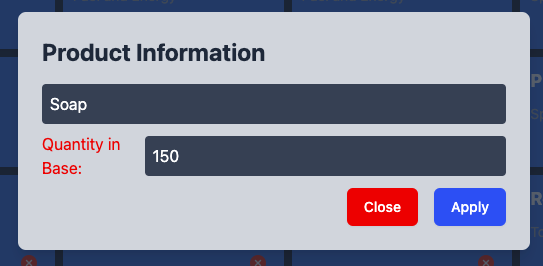
\includegraphics[width=0.5\textwidth]{img/admin-base-edit}
            \caption{Edit modal}
        \end{figure}

        Όταν κάνουμε hover εμφανίζεται ένα tooltip \textbf{Edit}, και αν το κλικάρουμε καλούνται οι πληροφορίες του αντικειμένου μέσω της \c{product\_info.php}, και μπορούμε να τις τροποποιήσουμε.
        Η τροποποίηση πραγματοποιείται μέσω της \c{onProductFound()}, η οποία εμφανίζει το αντίστοιχο modal και καλεί την \c{update\_product.php}.

        Μέσω του κόκκινου κουμπιού Χ, το αντικείμενο διαγράφεται.
        Για να διαγραφτεί ένα αντικείμενο, καλείται με AJAX το \c{delete\_product.php}.

        \subsubsection{Add an item}
            \begin{figure}[H] \noindent \centering
                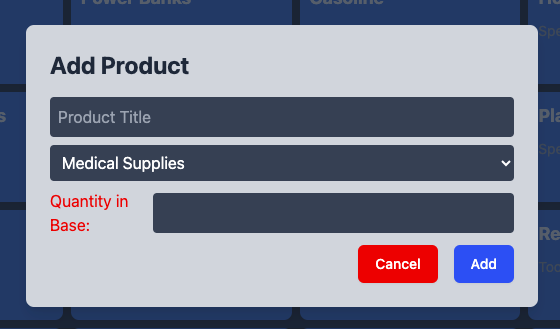
\includegraphics[width=0.5\textwidth]{img/admin-base-add}
                \caption{Add product modal}
            \end{figure}

            Το κουμπί \textbf{Add an item} ενεργοποιεί ένα modal με μια φόρμα για προσθήκη νέου προϊόντος.
            Για την επιλογή της κατηγορίας του προϊόντος χρησιμοποιείται το προηγούμενο JSON αρχείο, και όταν το καθορίσουμε και πατήσουμε \textbf{Add}, εκτελείται το \c{insert\_product.php}.
            Μετά την προσθήκη του προϊόντος, γίνεται update το περιεχόμενο της βάσης εκτελώντας ξανά το \c{item\_categories.php}.

        \subsubsection{Upload}
            \begin{figure}[H] \noindent \centering
                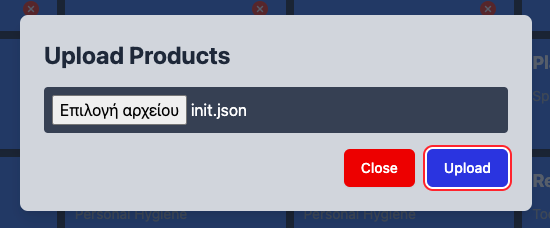
\includegraphics[width=0.5\textwidth]{img/admin-base-upload}
                \caption{Upload JSON modal}
            \end{figure}

            Το κουμπί \textbf{Upload} μέσω της \c{upload.js} ενεργοποιεί ένα modal, στο οποίο μπορούμε να ανεβάσουμε ένα JSON αρχείο και να αρχικοποιήσουμε ολόκληρη τη βάση.
            Υπάρχει ένα Event Listener που ενεργοποιείται με το κλικ στο κουμπί \textbf{Upload}, το αρχείο αποθηκεύεται σε έναν reader, και γίνεται ένα AJAX request στο \c{upload.php}.
            Η PHP ελέγχει αν το προϊόν υπάρχει ήδη (ελέγχοντας το \c{id} του), και αν δεν υπάρχει, τπ προσθέτει.

        \subsection{Map}
            Η σελίδα περιλαμβάνει μια οπτική αναπαράσταση των Requests, των Offer και των Rescuers σε έναν χάρτη.

            \begin{figure}[H] \noindent \centering
                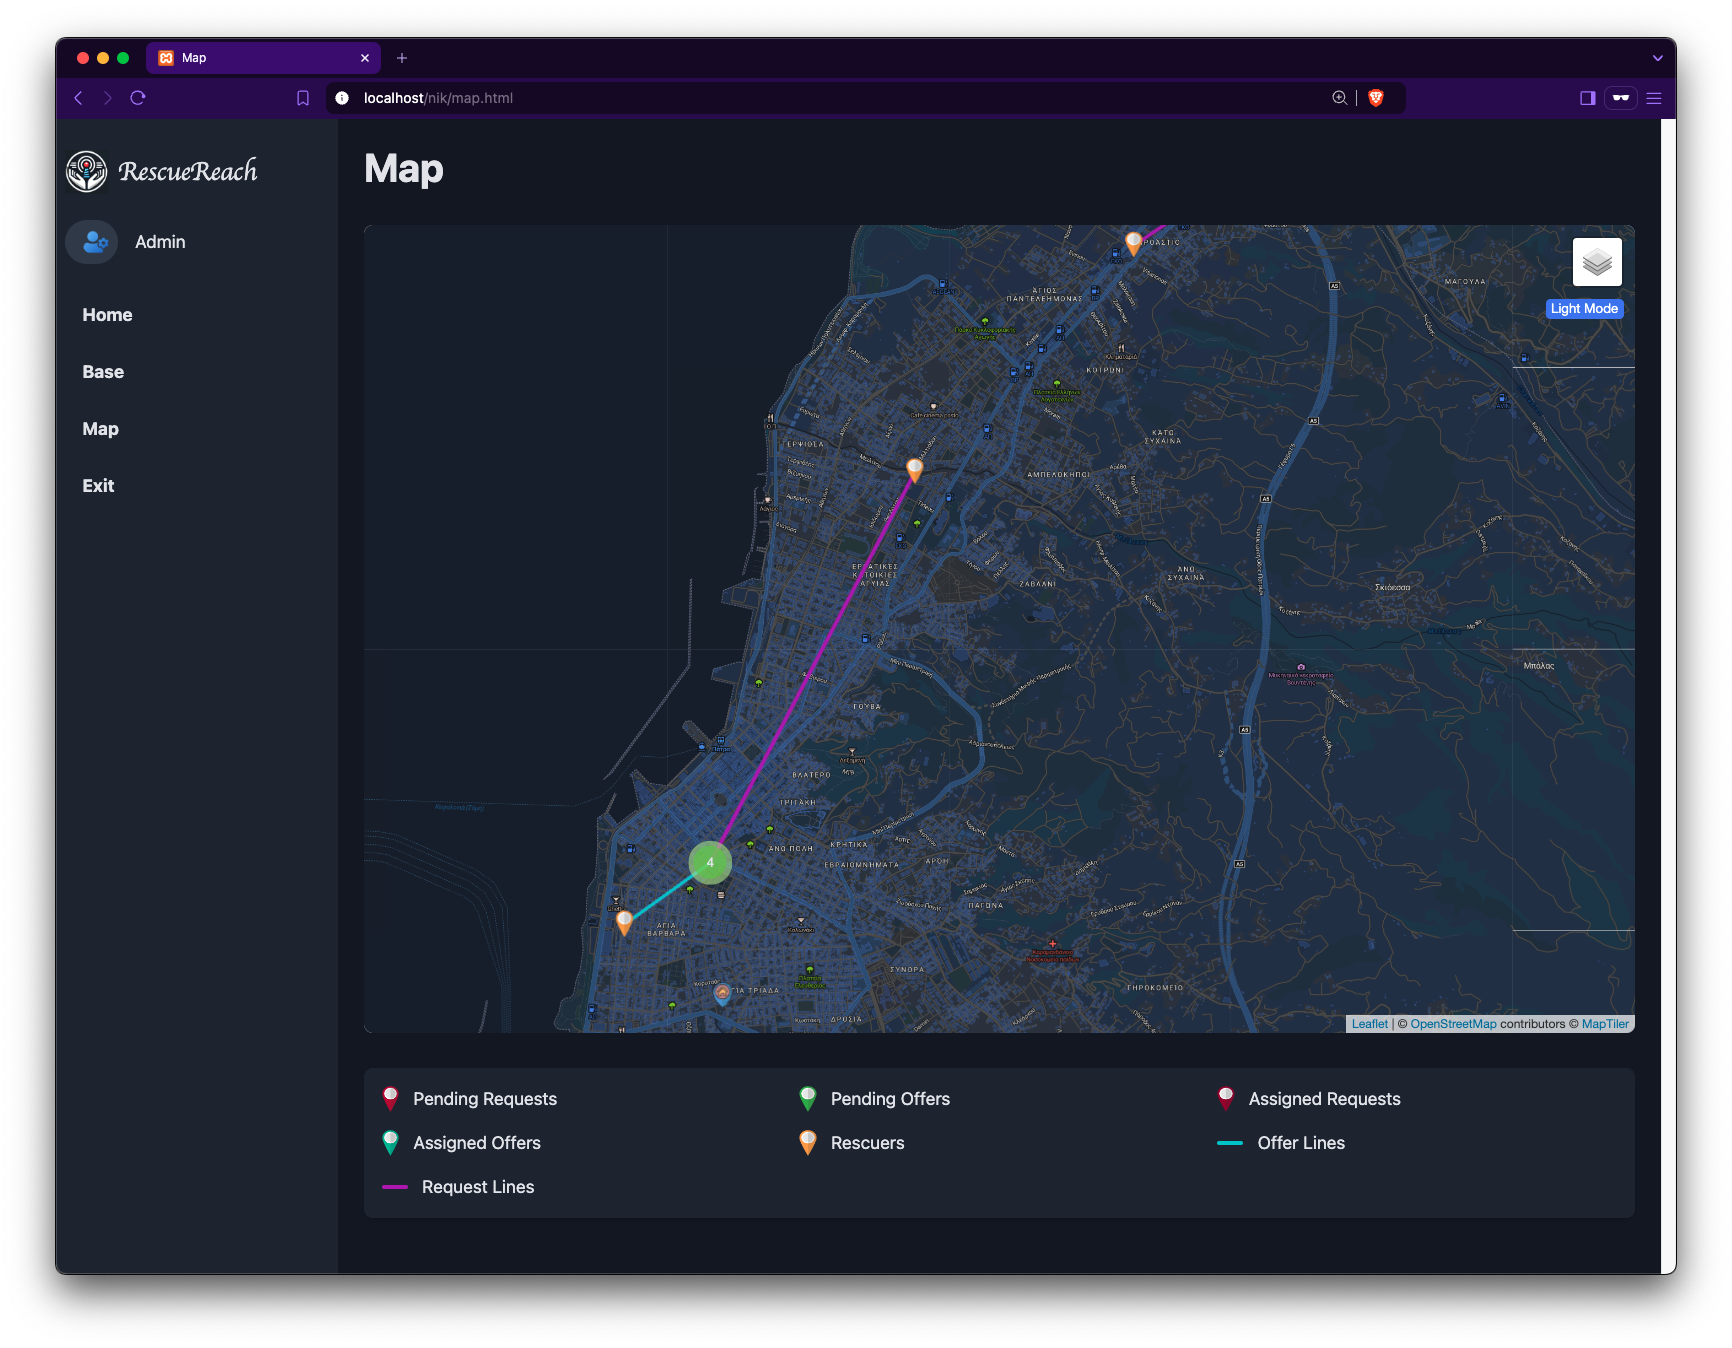
\includegraphics[width=0.8\textwidth]{img/admin-map}
                \caption{Χάρτης admin}
            \end{figure}

            Κατά τη φόρτωση της σελίδας, στο \c{map.js} τρέχουν οι συναρτήσεις